
\chapter{Radial Bias in large spatial scale optical imaging signal in the macaque Primary Visual Cortex}

\pagebreak

	\section{Summary}
	
	Neurons in the primary visual cortex are tuned to orientation and similarly oriented neurons are arranged in columns, with orientation columns arranged like spokes around a pinwheel. The different orientations are however not equally represented. Two different types of biases have been reported in the representation of orientations in the primary visual cortex, namely the oblique effect and the radial orientation bias. Electrophysiological and fMRI studies have shown a preponderance of the radial orientation in the primary visual cortex of mammals. However, optical imaging of intrinsic signals (OI), which are related to the fMRI signals do not show this radial bias. Here, OI signals on a spatial scale comparable to that of the fMRI signals were examined. The orientation selectivity of the spatially unfiltered, raw signal obtained from OI was compared to the radial angle and a significant radial bias was found in this signal. When a similar analysis was performed on a traditionally band-pass filtered OI signal, a much weaker radial bias was found. As the OI signal is predominantly due to synaptic and pre-synaptic activity, it is proposed that the global signal in OI corresponds to cortical inputs. If the cortical inputs are biased for only a small number of orientations, then this provides evidence for a model of orientation selectivity where orientation tuning of cortical neurons are sculpted from orientation biases encoded in a small number of broadly tuned channels.
			
\pagebreak

	\section{Introduction}
	
	Neurons in the primary visual cortex are tuned to orientation and the orientation tuned neurons are organised in columns. Hubel and Wiesel (1962) showed that neurons in Area 17 of cats were sharply tuned to orientation. These neurons were also grouped into neurons of similar orientation. Optical imaging studies in the cat A17 and 18 showed that the cortical orientation columns were organised as the spokes of a pinwheel, converging on the pinwheel centre (Bonhoeffer and Grinvald, 1991; Grinvald et al., 1986). Models of orientation selectivity and cortical architecture assume that neurons are equally tuned to all line orientations. However, studies suggest that there is an overrepresentation of some orientations in the visual system. Two types of orientation biases have been demonstrated in the visual system. The first is the oblique effect, which manifests as an underrepresentation of the oblique orientations while the horizontal and vertical orientations are overrepresented (see Appelle, 1972 for review). The second is the radial bias; where neurons are preferentially tuned to the orientation parallel to the line joining the centre of the receptive field to the centre of the visual field (Levick and Thibos, 1980). Both these biases have been reported in the macaques.
	
	Where the relationship between the receptive field location and visual field locus were studied, a radial bias has been reported every time. Early studies of biases in orientation representation in the cortex reported a strong oblique effect in electrophysiological studies (Chapman and Bonhoeffer, 1998; Coppola et al., 1998; DeValois et al., 1982; Kennedy et al., 1985; Leventhal, 1983; Li et al., 2003; Mansfield, 1974; Mansfield and Ronner, 1978; Orban and Kennedy, 1981, Payne and Berman, 1983; Pettigrew et al., 1968); which was congruent to the findings of a prominent oblique effect in behavioural studies reported in most species, from humans to octopuses (Appelle, 1972; Campbell et al., 1966; Furmanski and Engel, 2000; Rovamo et al., 1982). However, these studies examined the orientation preferences of neurons without studying their corresponding receptive field locations. Later studies that characterised the receptive field location with regards to the visual field locus all reported a radial bias in almost all species that were studied using electrophysiological studies (Levick and Thibos, 1980; Levick and Thibos, 1982; Maloney et al., 2014; Passaglia et al., 2003; Leventhal, 1983; Leventhal and Schall, 1983; Smith et al., 1990; Vidyasagar and Henry, 1990; Schall et al., 1986a; Schall et al., 1986b, Shou and Leventhal, 1989), fMRI imaging studies (Sasaki et al., 2006; Swisher et al., 2010; Mannion et al., 2010) and behavioural studies where subjects observed natural scenes instead of oriented gratings (Hanson and Essock, 2004).
	
	One of the key tools that have been instrumental in revealing cortical architecture is optical imaging of intrinsic signals (OI). Using OI, not only have the ocular dominance domains and orientation domains been visualised, but their relationships with each other have also been examined (Bartfeld and Grinvald, 1992). The haemodynamic change accompanying neural activity that is recorded using OI is akin to the BOLD (Blood Oxygen Level Dependent) response observed in fMRI (Menon et al., 1995; Logothetis et al., 2001). While the orientation biases studied using the fMRI BOLD responses reveal a radial orientation bias, only the oblique effect has been reported using OI (Chapman and Bonhoeffer, 1998; Coppola et al., 1998; Grabska-Barwinska et al., 2009).
	
	One reason for this discrepancy in these findings could be due to the spatial scale at which these signals are studied. The BOLD signal has a poorer spatial resolution compared to the OI signals, which is capable of resolving cortical columns (Churchland and Sejnowksi, 1988). The BOLD and OI responses predominantly consist of the pre-synaptic and synaptic activity with the extracellular, spiking activity forming a fairly small part of the response (Logothetis et al., 2001). Traditionally, images obtained using OI are band-pass filtered to reflect activity corresponding to a narrow spatial scale (between 100-500 microns). While this spatial filtering has the advantage of isolating the weaker, smaller spatial scale spiking activity, it has the disadvantage that by omitting the larger spatial scale activity, any information present at this spatial scale is lost. Here, we aimed to use the unfiltered larger spatial scale signal. We hypothesised that when this larger spatial scale signal is studied in the anaesthetised macaque striate cortex, we will find a bias for the radial orientation as has been reported in the fMRI studies. 
	
		
	\pagebreak
		
	\section{Methods}
	In this study, we imaged and recorded from the cortex of five, anaesthetised male macaques (Macaca nemestrina, 2-4 years old). All experimental procedures were approved by the Florey Institute of Neuroscience and Mental Health Animal ethics committee and conformed to the guidelines of the National Health and Medical Research Council’s Australian Code of Practice for the Care and Use of Animals for Scientific purposes.
		\subsubsection{Surgery and anaesthesia}
		Surgical procedures were as described in the methods section. Briefly, animals were anaesthetised using a Ketamine/Xylazine mixture (Ketamil, 15mg/kg, i.m., Parnell Laboratories, Australia; Cylazil, 2mg/kg, i.m., Troy Laboratories, Australia). Venous cannulation was performed on the cephalic vein to administer fluids and paralysant (Norcuron, initial bolus of 0.7 mg/kg followed by 0.2 mg/kg/hr, Organon Australia Pty Ltd) to the animal and a tracheostomy was performed to administer the anaesthesia (0.5-2\% Isoflurane in a mixture of nitrous oxide and oxygen (70:30)) during the experiment. The animal was placed in a stereotaxic frame and its head fixed using ear bars. During the experiment, the end-tidal CO2 (3.6-3.8\%), electrocardiogram, electroencephalogram and the core body temperature were all monitored. A craniotomy and durotomy were conducted over the location of the primary visual cortex (Horsley-Clarke co-ordinates: 24-34 mm posterior and 2-10mm lateral). The eyes were dilated by applying 0.1\% Atropine (Sigma Pharmaceuticals Pty Ltd, Australia) and rigid, gas permeable lens were introduced to prevent corneal drying and optical lenses and artificial pupil (4mm) were used to correct any refractive errors and reduce optical aberrations.
	
		\subsubsection{Optical Imaging of Intrinsic Signals}
		
		\paragraph{Setup}
		Optical imaging of intrinsic signals was used to obtain the haemodynamic change related to the neural response to orientation stimuli. The OI setup involved two camera lenses (2 x Pentax lenses, f=50 mm) arranged in a tandem fashion (Frostig et al., 1990) connected to a CCD camera (Teli CS8310B). The tandem lens arrangement allowed us to choose a narrow plane of focus. An LED light source was used to illuminate the cortical surface. Before stimulus presentation, a high contrast, ‘green image’ of the surface of the cortex was obtained by illuminating the cortical surface with a green light (filter wavelength=545 nm). This provided us with cortical landmarks which were later used in determining the locations for electrode tracks of topographical recordings. Following this, the camera was focussed between 550-700 microns beneath the surface of the cortex and a red light filter (wavelength =630 nm) was used to illuminate the cortex. 
		
		\paragraph{Stimulus and data collection}
		
		During the experiment OI maps were obtained in response to visual stimulation. Visual stimulus was generated using the visual stimulus generator (SDL, Cambridge Research Systems, UK) and presented on a Barco monitor (Reference Calibrator plus; Barco Video and Communications, Belgium).  The monitor was positioned at 57 cm from the animal. The stimulus presented was a full field, square-wave, bidirectional, drifting grating (SF= 1-4 cpd, TF= 1.5 Hz, Contrast= 100\%). The orientation of the grating changed sequentially in 22.5 degree steps from zero to 157.5 degrees. A zero degree grating was a horizontal grating moving bidirectionally. The stimulus was presented for 7.3 seconds followed by an interstimulus interval of 10 seconds where the animal viewed a blank screen. 18 frames, each 400 ms long were collected for each stimulus presentation. The signal to noise ratio was enhanced by acquiring data over 50 trials collected in 10 blocks of 5 trials each. Where possible, given the condition of the imaged area and the animal, the experiment was repeated for a second time. Using the OI data acquisition system, each block was exported as a MATLAB® file. Each individual frame in a block was the average of that frame over 5 trials. Analysis was conducted on the exported MATLAB files.
		
		\paragraph{Image Analysis}
		
		Of the 18 frames collected, the mean of 14 frames (frames 3-16) was calculated for individual blocks in each stimulus condition. The first frame was then subtracted from the averaged frames for each stimulus condition. The mean of 10 blocks was then calculated. This gave us the unfiltered single condition maps (unfiltered SCMs). Traditionally, when analysing the images obtained using optical imaging of intrinsic signals, the unfiltered SCMs are band pass filtered using the method described in figure (Refer to method figure). The unfiltered map is first low pass filtered using a large spatial filter (Gaussian filter, sigma= 312.5 microns). This removes the low frequency information. By subtracting this low pass image from the original image, we preserve only the high spatial frequency information (high-pass SCMs). The high pass SCM is then smoothed with a gaussian filter with a smaller sigma value (100 microns). This is the band pass filtered single condition map or more commonly just referred to as the single condition map (these will be referred to as filtered SCMs throughout this thesis). The filtered SCMs are then vector averaged to look at the angular mean of individual pixels (Swindale, 1988). This will produce the traditional filtered orientation tuning maps. In our study, we also vector averaged the unfiltered SCMs. We called the maps derived this way the unfiltered orientation maps.
		
		\subsubsection{Topographical recordings}
		High impedence tungsten microelectrodes (6-12 MOhm, FHC Inc, ME) were used to record from predetermined locations on the imaged cortical surface. The analog signal was amplified and filtered (AM Systems model 1800, Washington; Gain = x10,000; Band pass between 300 and 3000 Hz). The filtered signal was then visualised using an oscilloscope and fed through an audio speaker to aid in plotting the receptive fields. First the foveal location (if visible) and the optic nerve with blood vessel markers were plotted using a back-projecting fundus camera. Then the locations of the receptive fields were carefully hand plotted using handheld stimuli from at least 3 locations in the imaged area. In between each electrode penetration, where possible, the location of the fovea and optic nerve head were replotted in order to account for eye movement. At six locations, the signal obtained from the electrodes and the filtered signals were digitzed (12.5 - 22.5 kHz, CED; Cambridge Electronic Systems, UK) and stored for later analysis.
		
		\subsubsection{Multi-electrode array recordings}
		In one animal, we used a 16 channel, linear, multi-electrode array (NeuroNexus Technologies Inc, USA) to record from the cortex. The array was inserted at an angle within the supragranular layers of V1. The individual electrode on the multielectrode array were separated by 100 microns. The array was connected to a pre-amplifier (RA16PA, Tucker-Davis Technologies, USA) through a headstage (RA16AC). The signal was amplified (x 10000) and filtered (2.2 Hz- 7.5 kHz) was applied and the resultant signal was digitized (12.5kHz) using the OpenEx software (TDT, USA). The digitized signal was further digitally filtered between 2.2Hz and 100 Hz, and down-sampled to 1017.3 Hz to obtain the LFP signal and between 300-3000 Hz to obtain the multi-unit recordings.
		
		\subsubsection{Stimulus for electrode recordings}
		To make topographical recordings, a handheld stimulus was used. The orientation, direction and speed of the stimulus movement were all varied so that the neuron was ideally stimulated. Following this, the receptive fields of the neurons were hand-plotted and used for further analysis.
		
		For the single electrode recordings and linear array recordings, a bi-directional moving bar (10o x 0.5o bar, contrast = 100\%, speed= 2.5- 5o/s), whose orientation changed incrementally from -90o in steps of 20o was used. The responses were recorded for 9 orientations with bars moving in 2 directions (a total of 18 directions) over 10 trials. The monitor used to present the stimuli and software used to generate the stimuli were the same as described for optical imaging.
		
	\subsubsection{Data Analysis}
	
		\paragraph{Analysis of electrophysiological recording}
		
		For both the single electrode and the linear array recordings, multi-unit activity and LFPs were analysed to get the optimum orientation at a recording site. For recordings made using single electrodes, the Spike 2 software (Cambridge Electronic Systems, UK) and for linear array recordings, the Open Ex Software (TDT, USA) were used to apply digital filters to separate the signals into LFP (between 20 and 70 Hz) and multiunit activity (between 300-3000 Hz).  The LFP signal corresponding to each stimulus direction was averaged across 10 trials using custom code written in MATLAB. The difference between the peak and the trough of LFP signal at each orientation, over the location of the receptive field, was the maximum response at this orientation. These values were used to generate the polar plots and calculate the circular mean (as calculated by Swindale, 1998; See Appendix for code) at each of the recording sites. For multi-unit activity, a threshold was placed using the spike 2 software and any spike the was greater than this signal was collected into PSTHs and SDFs were made. The peak firing rate at each direction of movement was used to generate polar plots and calculate the circular mean of the data.
		
		\paragraph{Determing radial orientation- receptive field locations}
		
		In order to determine the azimuth and elevation of receptive fields obtained during the experiment, the Cartesian co-ordinates of the foveal location was set as (0,0). The horizontal and vertical distances of the receptive field centre from the foveal location were calculated. The azimuth and elevation of receptive fields were then calculated as the horizontal and vertical angles subtended by the animals’ eyes to the receptive field centre. If there were eye movements during the experiment, (0,0) was re-assigned to the new foveal location. Receptive field locations were replotted in relation to foveal locations plotted closest to the recording in order to get as accurate a receptive field location as possible. This then allowed us to accurately determine the azimuth and elevation of the receptive fields.
		
		Using the receptive field locations thus calculated, we used the eccentricity, azimuth and elevation values to calculate iso-azimuthal and iso-elevation lines on the cortex. We used previously published magnification factor calculations in the macaque cortex (Dow et al.,1981) to calculate the magnification factor —degrees in visual space one would traverse if we moved 1 mm in cortical space and the inverse magnification factor; how far one needs to move on the cortex to traverse 1 degree in visual space, given the eccentricity of the receptive fields. These values were used to calculate the azimuth and elevation of points on the cortex that were spaced 15 pixels (375 microns) apart. The radial angle of each of the points was calculated given the azimuth and elevation of their RF locations and averaged to calculate the average radial angle of the imaged area.
		
		\paragraph{Defining a region of interest}
		As described above, the azimuth and elevation of points on the cortex that were 375 microns were calculated. 30 x 30 pixel squares around these points were defined as Regions of interest (ROIs). The difference between the average optimum orientation of the individual pixels in the ROIs and the radial angle of the ROI centre was calculated for both the unfiltered and filtered orientation maps (See fig\ref{fig:roi}).
		
			\begin{figure}[H]
			
			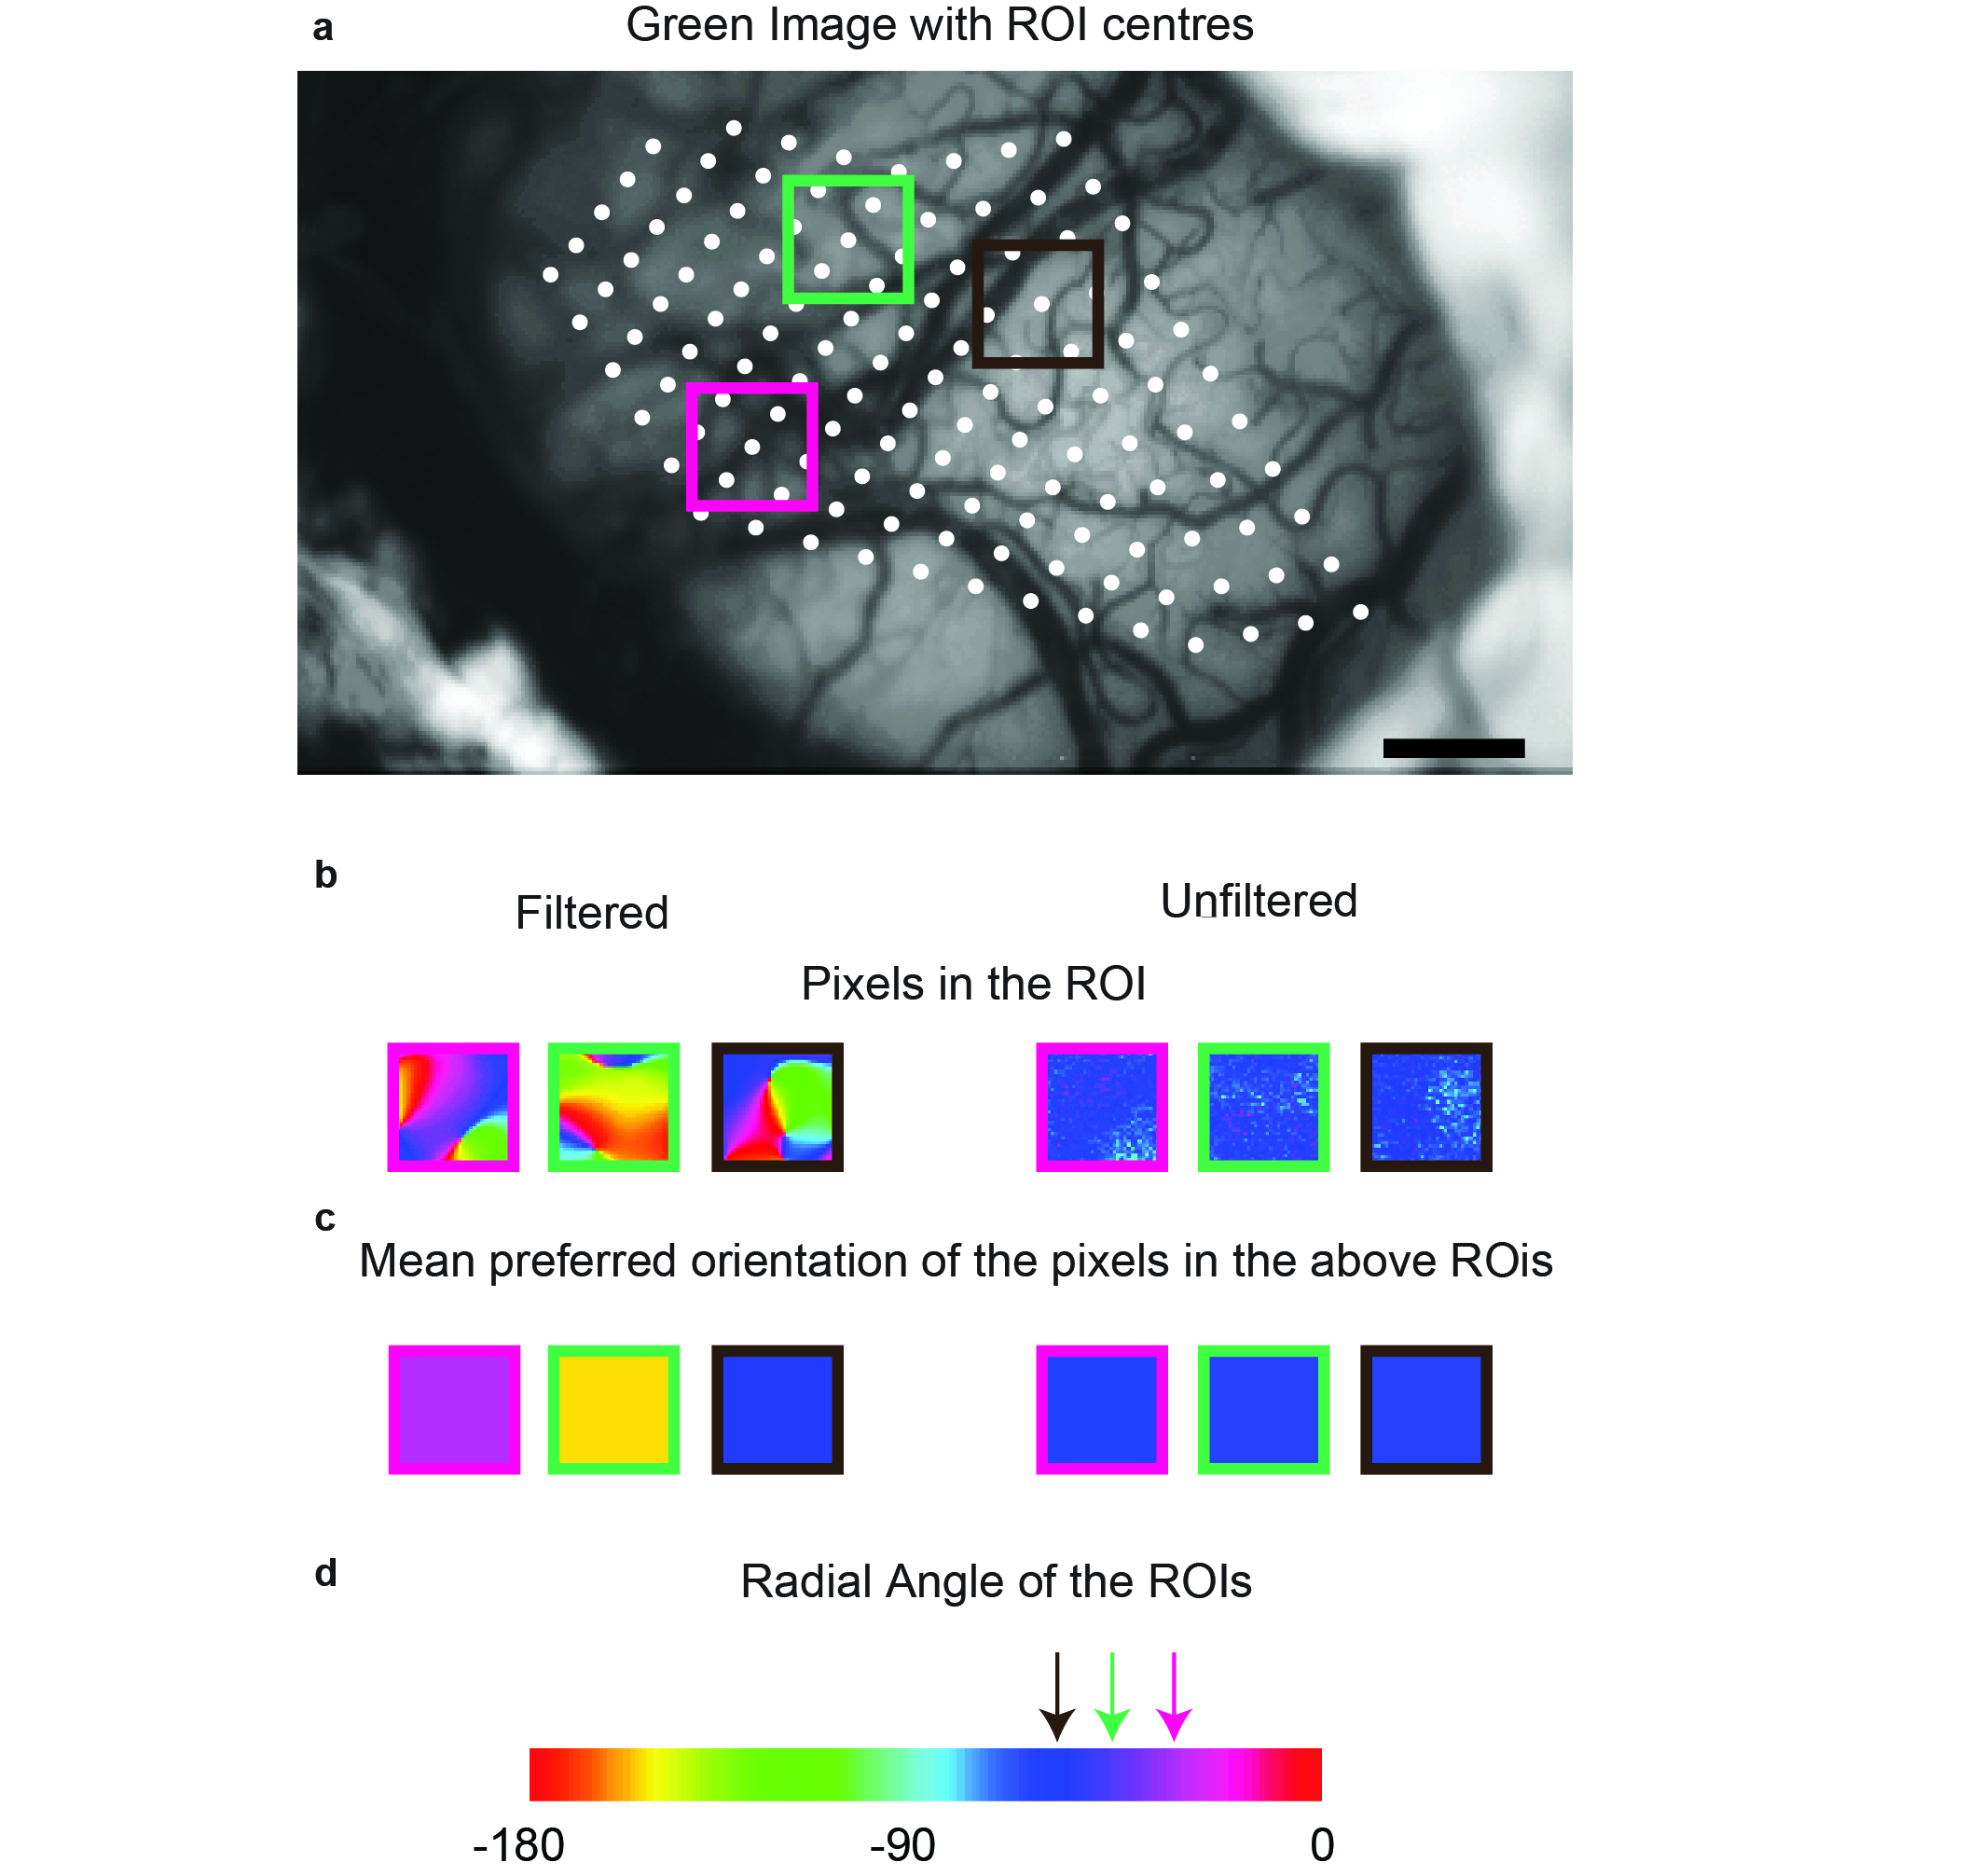
\includegraphics[width=\linewidth]{rb/FinalFigures/ROI.jpg}
			\caption{The generation of Regions of Interest (ROIs). a) the green image from the representative animal. The white dots are the centres of the ROIs. The ROIs were placed 15 pixels apart. Three ROI centres were randomly chosen and the region that is used for analysis is shown by the three coloured squares. b) shows the individual pixels in the filtered and the unfiltered conditions in the respective ROIs. c) shows the average orientation of the pixels in the ROIs. d) is the pseudo-color scale used to represent the different orientations in the orientation tuning maps and the pixels in the ROI. The three coloured arrows indicate the radial angle of the corresponding ROIs.}
			\label{fig:roi}
		\end{figure}
		
		\paragraph{Single Pixel Analysis}	
		
		The ROI analysis was used to determine if any of the cortical inputs were dominant in the larger spatial scale. To see if such bias was present at a single pixel level, we also compared the orientation tuning of single pixels to the radial bias of the imaged area. Accordingly, the optimum orientation of the individual pixels was subtracted from the mean radial orientation of the imaged area for the unfiltered and filtered maps. 
		
		\paragraph{Adjusting for sample size in single pixel analysis}
		
		During the single pixel analysis, individual pixels from orientation maps in five animals were examined. This amounted to a large number of pixels (10$^5$ pixels). In order to make sure we were not detecting an insiginificant effect made significant by sample size, we randomly resampled with replacement from the distribution of pixels in both the filtered and the unfiltered conditions to see if an effect could be observed at smaller sample sizes. We used two sample sizes (40 and 1000) sampled 1000 times and calculated the chi-square of the 1000 trials. The mean and the 95\% confidence intervals of the chi-square value from 1000 trials were calculated. If the upper limit of the 95\% CI of the chi-square value was lower than the 5\% critical value, then the distribution of the single pixel differences was not significantly different from a uniform distribution in the majority of trials. If the lower limit of the 95\% CI was higher than the 5\% critical value, then the distribution of the single pixel differences was deemed significantly different from a uniform distribution in the majority of trials.
		\pagebreak
		
	\section{Results}
		We recorded from 5 monkeys (Macaca fascicularis, all male, aged between 2 and 5 years). In 3 monkeys, we imaged and recorded from the left hemisphere and in the other 2, from the right hemisphere. In all animals, OI signals were first recorded from the respective hemisphere; following this, topographical recordings were made. In 2 macaques, LFP recordings were made using single electrodes and in one macaque, the multi-electrode, linear array was used for recordings.
	
		\subsubsection{Single Condition Maps}
		As a first step in processing the results of OI, SCMs were made. The SCMs for the unfiltered and filtered maps from one representative animal are presented in figure 2a and b respectively. The orientation of the stimulus is shown above the respective SCM. The SCMs show that there is more activity overall in orientations closer to the radial orientations (denoted by the star) in the unfiltered maps (i.e. the overall map is darker). No such trend is visible in the filtered maps. Distribution of the intensities of the pixels of inverted SCMs (So that darker pixels have a greater intensity value) are presented in figure 2c. The line above the boxplots indicates the range of radial orientations of the imaged area in this animal. As observed in the SCMs, there is a peak at the radial orientation in the unfiltered maps while the distribution of the filtered pixels show no such trend.
			
						\begin{figure}[H]
							
							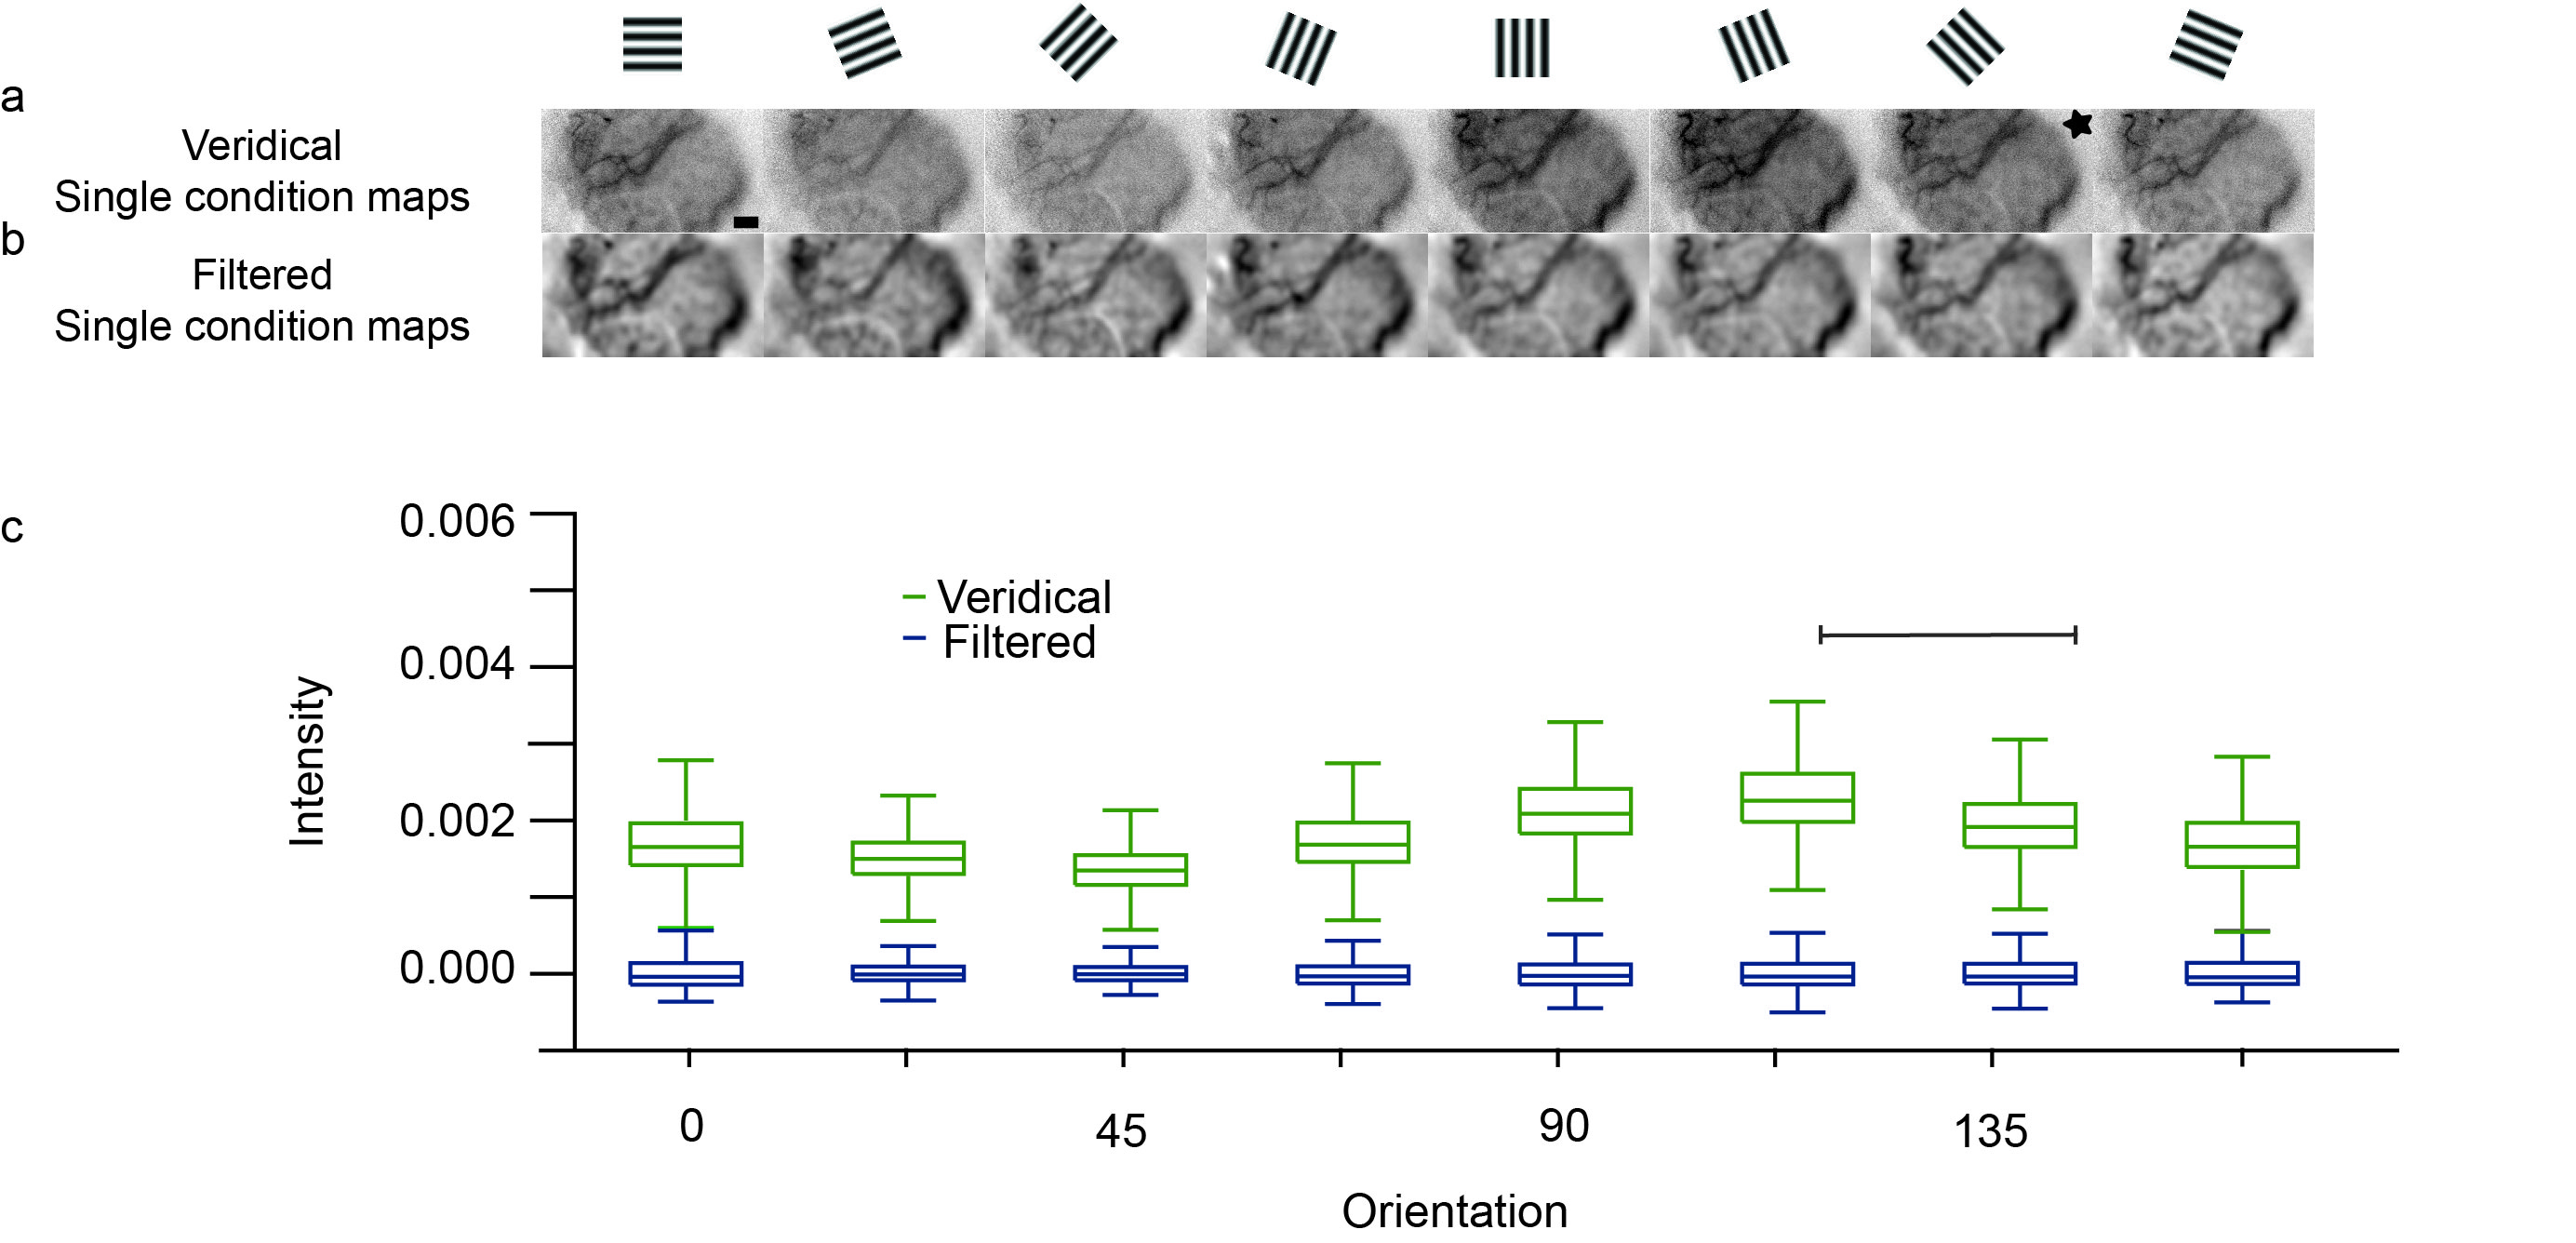
\includegraphics[width=\linewidth]{rb/scms.jpg}
							\caption{Distribution of pixels in unfiltered and filtered SCMs. (a) and (b) are the unfiltered and filtered SCMs. The stimulus orientation corresponding with each SCM is presented in the row above. The star denotes the orientation closest to the radial angle. Scale bar is 1mm. (c) is the boxplot of the distribution of the intensity of pixels in the unfiltered and the filtered maps. The line indicates the range of radial angles in the imaged area.}
							\label{fig:scm}
						\end{figure}
					
		\subsubsection{Orientation Tuning Maps}
			The unfiltered and filtered SCMs shown in figure 2a and b were vector averaged (Swindale, 1998) to produce the unfiltered and the filtered orientation maps in fig.\ref{fig:rep}. Figure \ref{fig:rep}a is the green image of the cortical surface with surface blood vessel landmarks. The different symbols correspond to the location of electrode tracks. The receptive field locations of the electrode tracks are shown in figure \ref{fig:rep}b. The polar plot corresponds to the orientation of a layer 2/3 neuron recorded from the location indicated by the diamond. The orientation of this neuron estimated using electrophysiological recording was 65.61$^o$; which was less than 22.5$^o$ away from the orientation of the neuron estimated using optical imaging was 86.89$^o$. The pseudo colour scale on the outside of the Cartesian scale is the same scale used in parts c and d. Figure \ref{fig:rep}c shows the filtered orientation maps and Figure \ref{fig:rep}d, the unfiltered orientation maps obtained during two repeats of the experiment. The filtered orientation map shows classical orientation domains that converge at a pinwheel centre, while the unfiltered orientation map is dominated by one orientation. This orientation corresponds to the radial orientation of the receptive fields in figure \ref{fig:rep}b; i.e. if we draw a line from the center of fixation to the center of the receptive field and extend it to the outer colour scale, we will observe the same colour as that seen in the unfiltered maps. Results for the unfiltered maps are presented in a similar fashion for all the animals in our study in figure 4.
			
							\begin{figure}[H]
								
								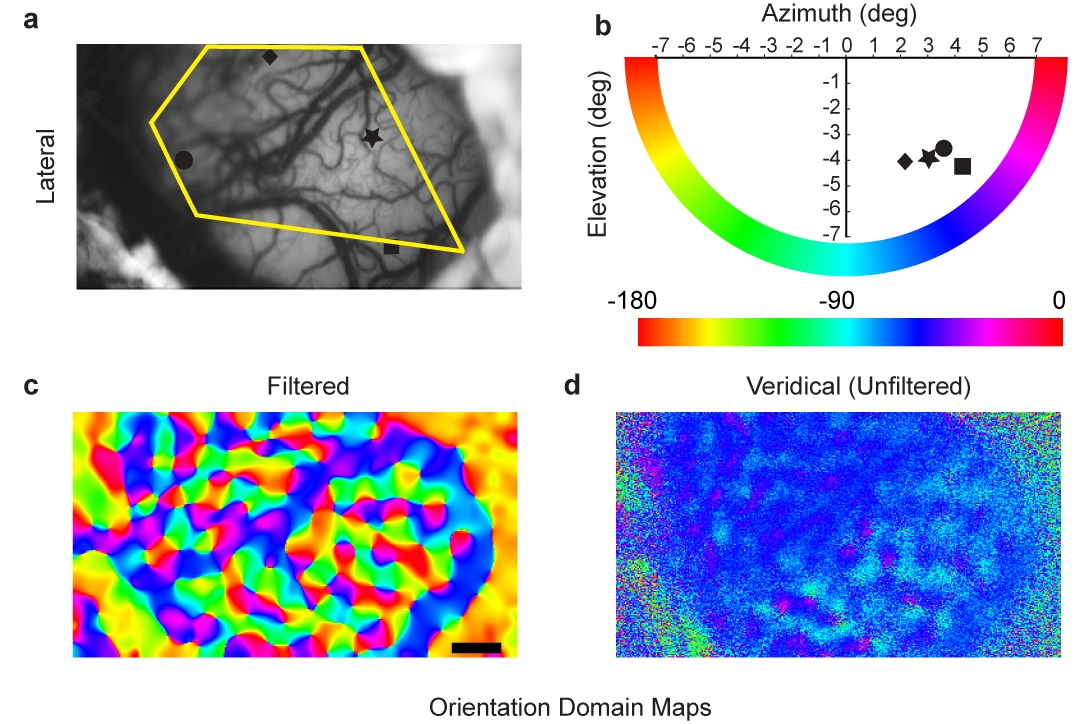
\includegraphics[width=\linewidth]{rb/figure1.jpg}
								\caption{Orientation tuning of the filtered and unfiltered signals. a) the cortical green image showing the cortical landmarks and the location of the electrode tracks. b) the different symbols indicate the receptive field location of the respective electrode tracks. The polar plot indicates the orientation of the unit obtained using single unit recording. The outer pseudo-color scale is the same as the one used in c and d. c) and d) are the filtered and the unfiltered maps.}
								\label{fig:rep}
							\end{figure}
			
			
			\begin{figure}[H]
				
				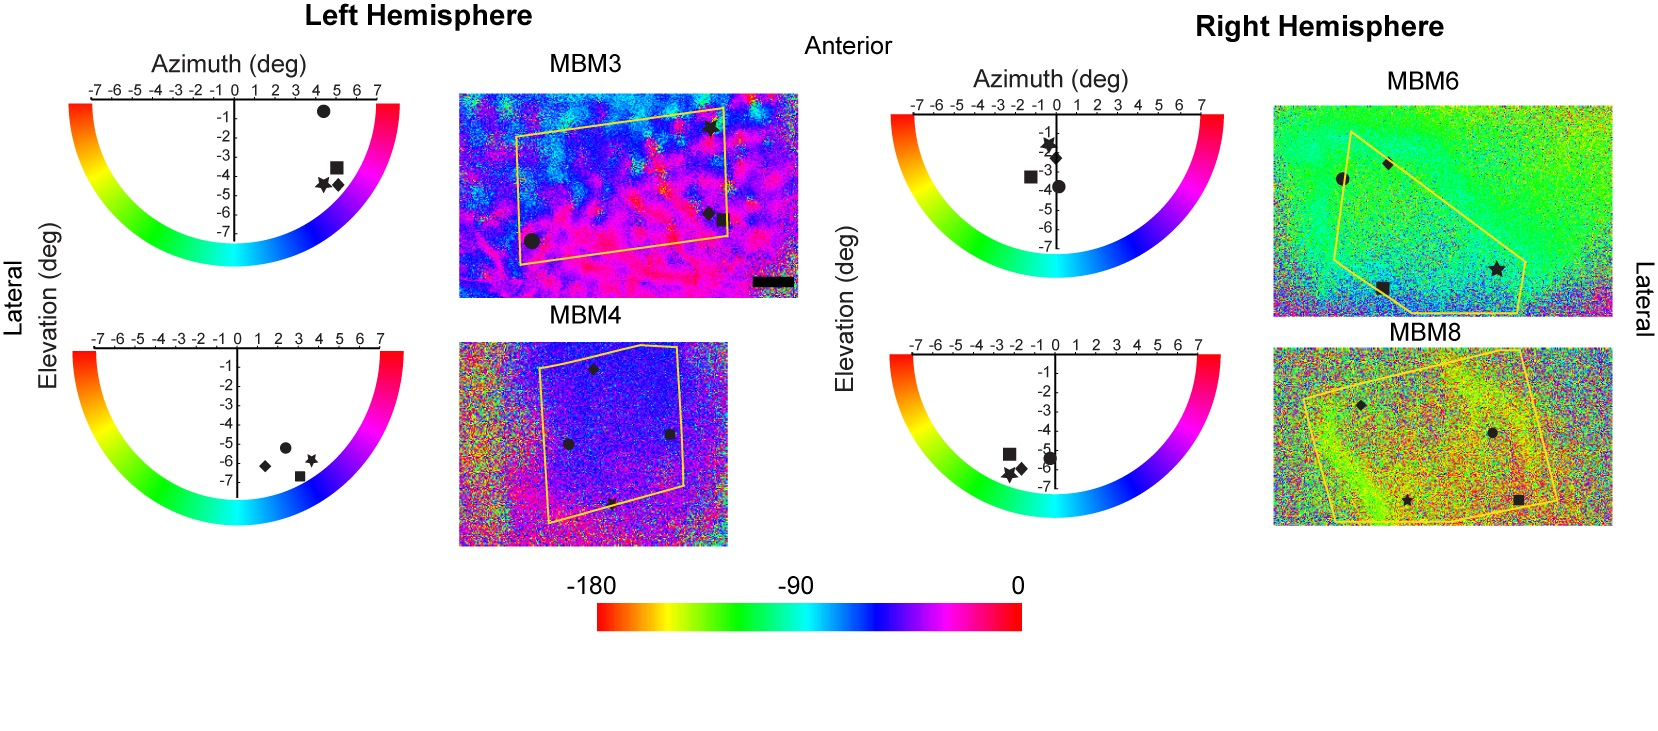
\includegraphics[width=\linewidth]{rb/figure2.jpg}
				\caption{The receptive field location, veridical and filtered orientation tuning maps of  all the animals (except that showed in figure \ref{fig:rep}) used in our studies. The conventions are as explained figure \ref{fig:rep}.}
				\label{fig:all}
			\end{figure}
							
		\subsubsection{Comparing the radial orientation and optimum orientation of ROIs}
		The optimum orientation of the pixels in the ROI and the radial angles of the ROIs were calculated and compared as described in the methods for 456 ROIs. Most ROIs were tuned to the radial orientation in the unfiltered maps. In the filtered maps, this bias for the radial orientation in the ROIs was observed to a smaller extent. Figure \ref{fig:roihist}a shows the distribution of the absolute differences between the optimum and radial orientations of the ROIs for the unfiltered and filtered orientation maps. The distribution of differences was significantly different from a uniform distribution for the unfiltered ($\chi^2$= 505.28; df=3; p$<$0.0001) as well as the filtered conditions ($\chi^2$= 35.21; df=3; p$<$0.0001). The filtered and the unfiltered distributions were also significantly different from each other ($\chi^2$= 283.01; df=3; p$<$0.0001).
			
			\begin{figure}[H]
				
				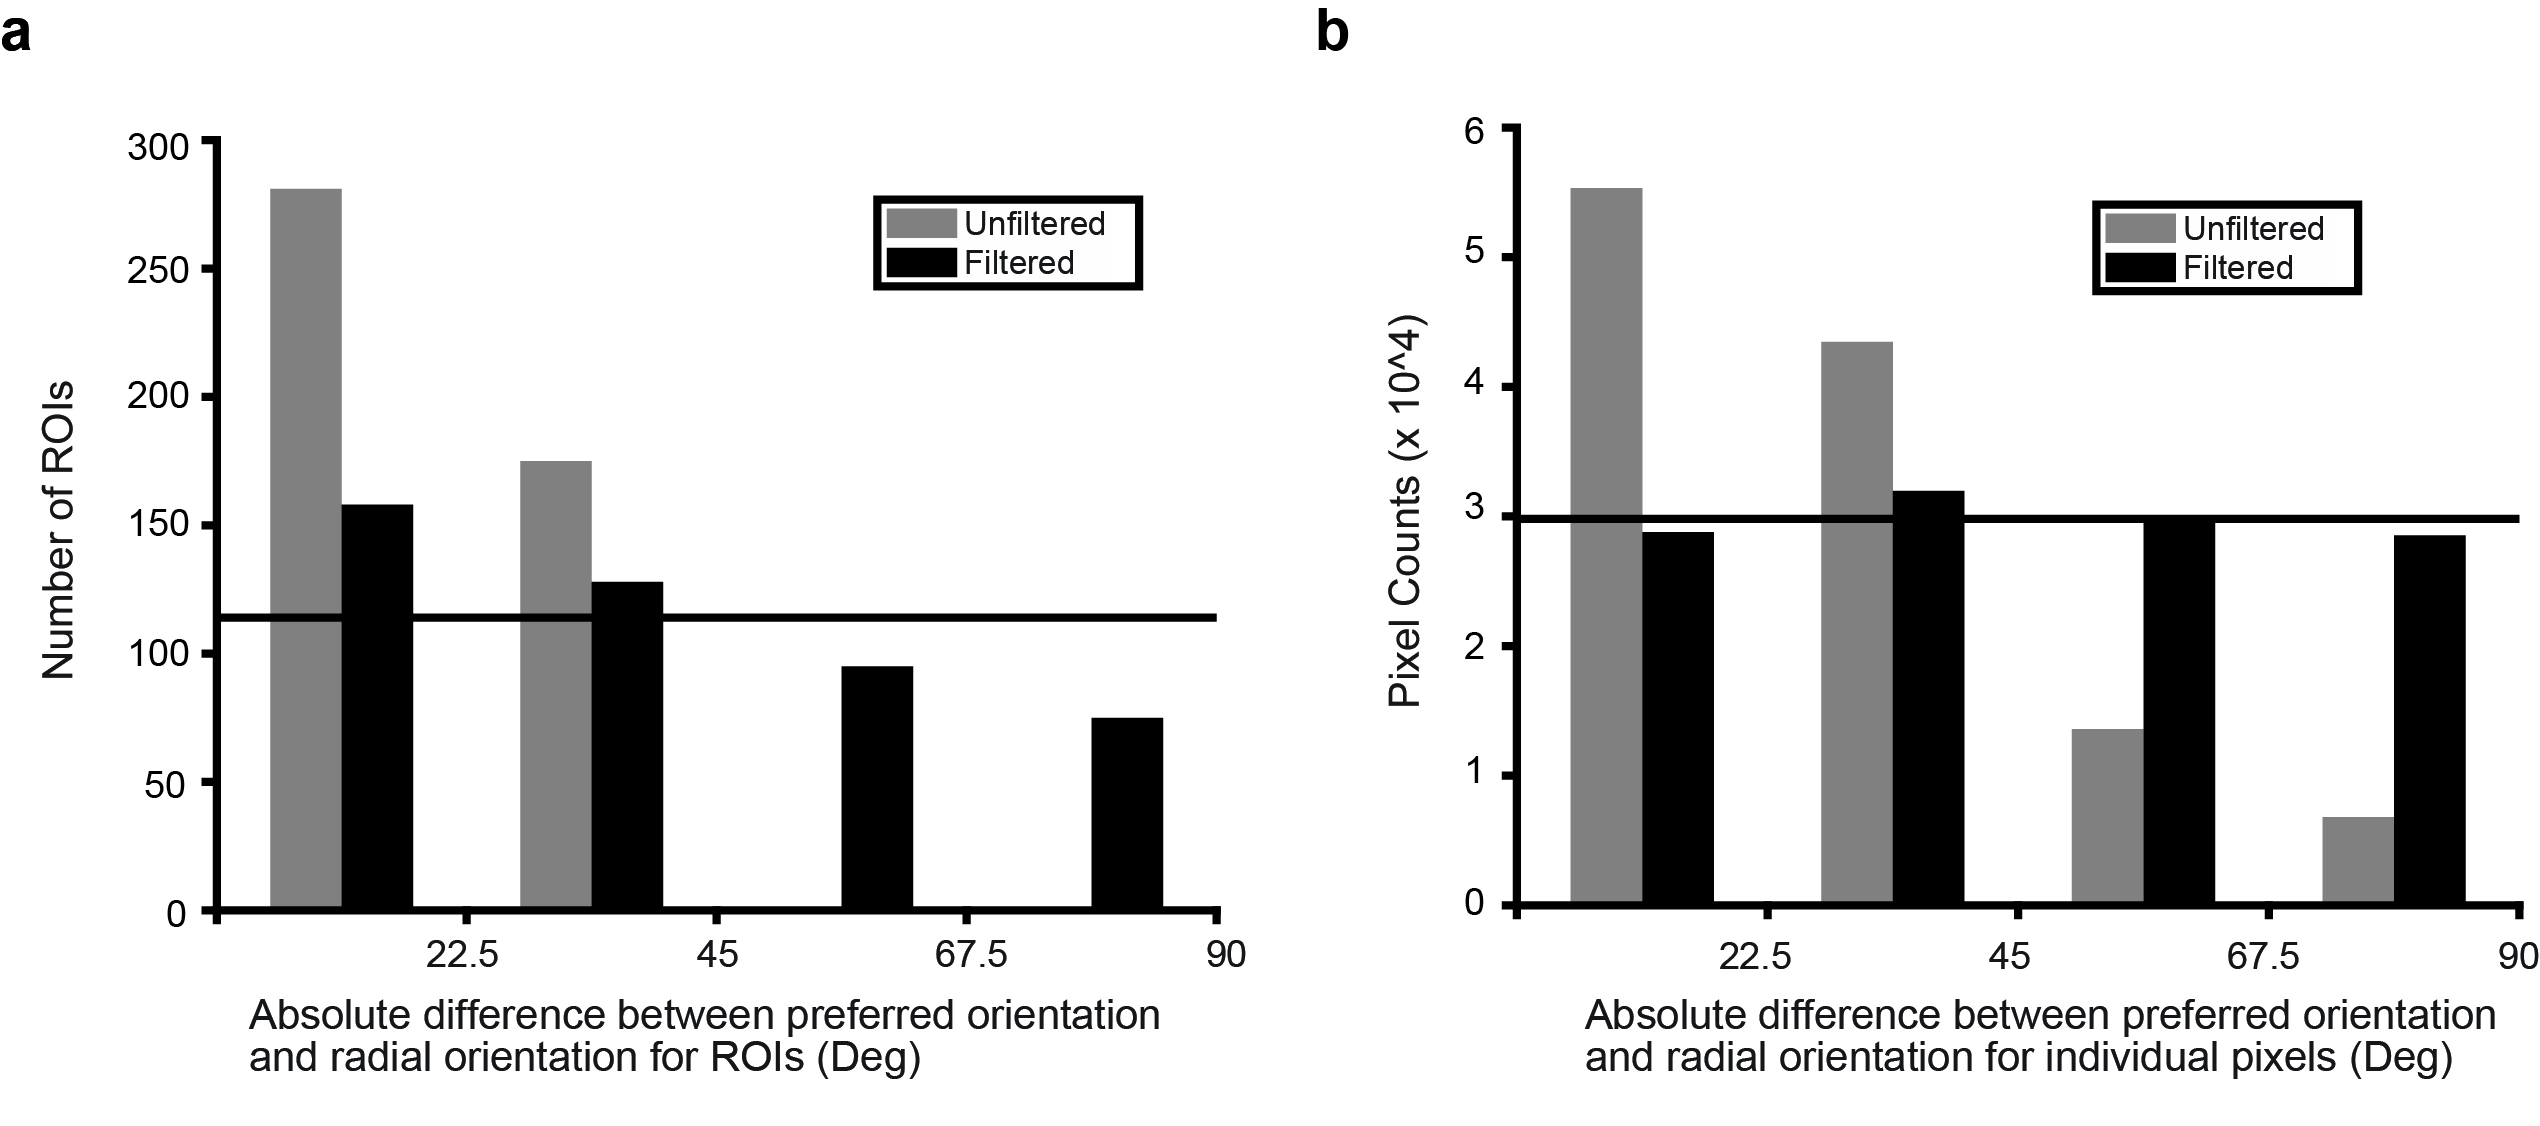
\includegraphics[width=\linewidth]{rb/FinalFigures/ROIhist.jpg}
				\caption{a) The absolute difference between the optimum orientation and the corresponding radial angle of the ROIs. Horizontal line is the distribution we would expect if the distribution was uniform. Total number of ROIs= 456. b) The distribution of absolute differences between the optimum orientation of single pixels and the radial angle of the imaged area.}
				\label{fig:roihist}
			\end{figure}
		\subsubsection{Comparing the radial orientation and optimum orientation of single pixels}
		The ROIs average the signal over 900 pixels (30X30 pixel square). We also examined the difference between the optimum orientation of individual pixels and the mean radial orientation of the imaged area to see if the radial bias was also present at the single pixel level. The single pixel differences showed that most pixels in the unfiltered condition were tuned to the radial orientation. Figure 6 shows the distribution of differences between the individual pixels and the mean radial orientation for the unfiltered and the filtered conditions. Once again, there was a strong peak between 0 and 22.5 degrees in the unfiltered condition. When compared with a uniform distribution (indicated by the horizontal line); the distribution of the differences for the unfiltered condition was significantly different (n= 119229; ($\chi^2$= 54691; df=3; p$<$0.0001). No clear anisotropies were observed in the filtered single pixel responses although the overall response was still significantly different from a uniform distribution (n= 119229; ($\chi^2$= 246.24; df=3; p$<$0.0001). The distribution of the filtered differences were also significantly different from the unfiltered differences (n=119229; ($\chi^2$= 54077; df=3; p$<$0.0001). We did not find any significant biases for horizontal and vertical orientations in either the ROI or the single pixel data.	
			
		For the single pixel analysis, as we used a large sample size (119229), the chi-square test, will always give a significant result regardless of the effect size. In order to address this issue, we used a repeated sampling paradigm, where smaller samples were randomly chosen from the overall pixel population and chi-square tests were performed on these distributions. We used two sample sizes (either 40 or 1000) and sampled 1000 times (1000 trials) from the overall population. The results indicate that the radial bias observed in the unfiltered maps were strong and were observed even in the condition with a relatively small sample size of 40 pixels (mean $\chi^2$= 21.09; CI= [20.95, 21.24];$\chi^2$ critical =7.05). There was also a statistically significant radial bias observed with the larger sample size of 1000 pixels for the unfiltered maps (mean $\chi^2$= 461.93; CI= [461.68, 462.19]; $\chi^2$ critical =7.05). For the filtered maps however, while the distribution was significantly different from a uniform distribution when sample size was 119229, the distribution was not significantly different from a uniform distribution when the sample size was 40 (mean $\chi^2$= 2.99; CI= [2.84, 3.13]; $\chi^2$ critical =7.05) or 1000 (mean $\chi^2$= 5.18; CI= [4.92, 5.44]; $\chi^2$ critical =7.05). These results suggest that the statistically significant result shown for a sample size of 119229 was most likely due to the large sample size. A summary of these results are presented in figures \ref{fig:s40} and \ref{fig:s1000} for the 40 and 1000 pixel samples respectively.
			
				
				\begin{figure}[H]
					
					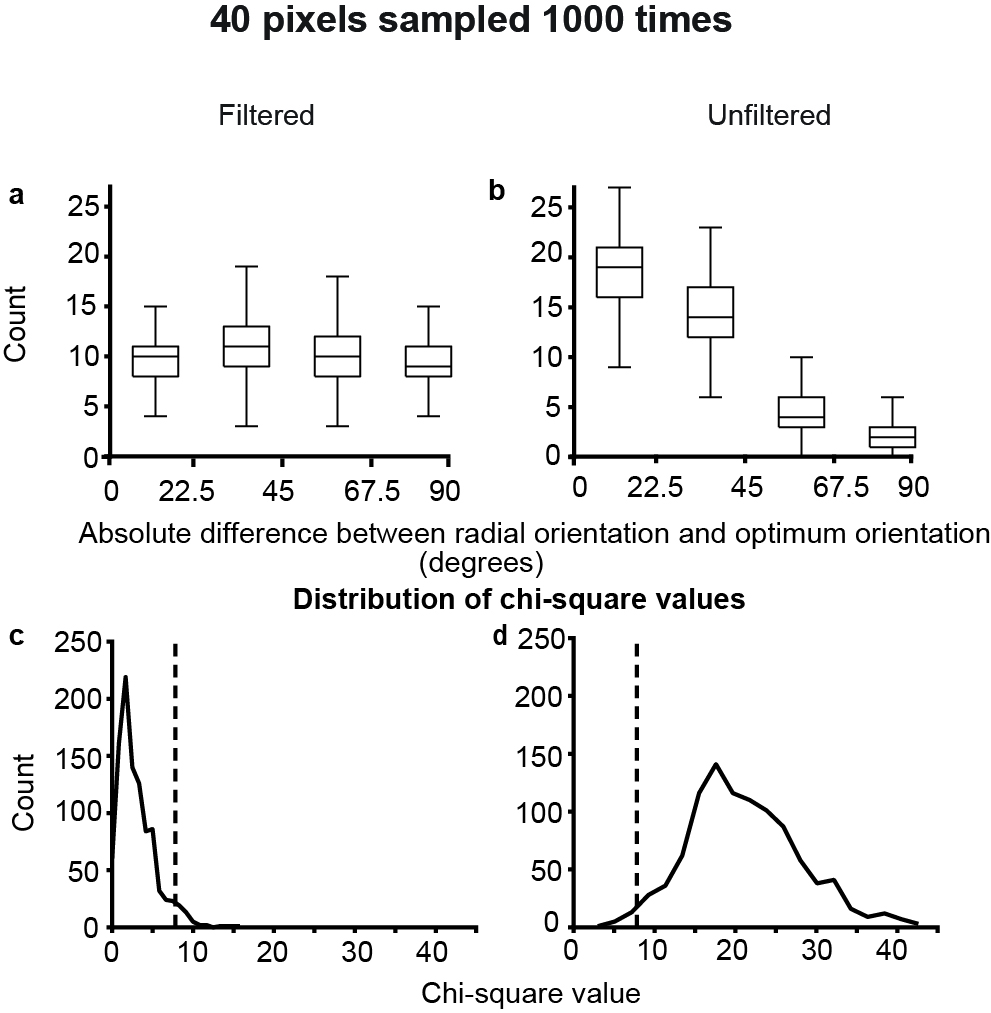
\includegraphics[width=\linewidth]{rb/FinalFigures/s3.jpg}
					\caption{Results of the random simulation experiment with 40 pixels sampled 1000 times. a) and b) show the distribution of the preferred orientation of the single pixels, centered on the radial orientation in the filtered and unfiltered conditions respectively. The boxplot indicates the distribution of the values over 1000 trials. c) and d) show the distribution of χ2 values for 1000 trials. The dotted lines indicate the location of the critical value for p=0.05.}
					\label{fig:s40}
				\end{figure}
				
				\begin{figure}[H]
					
					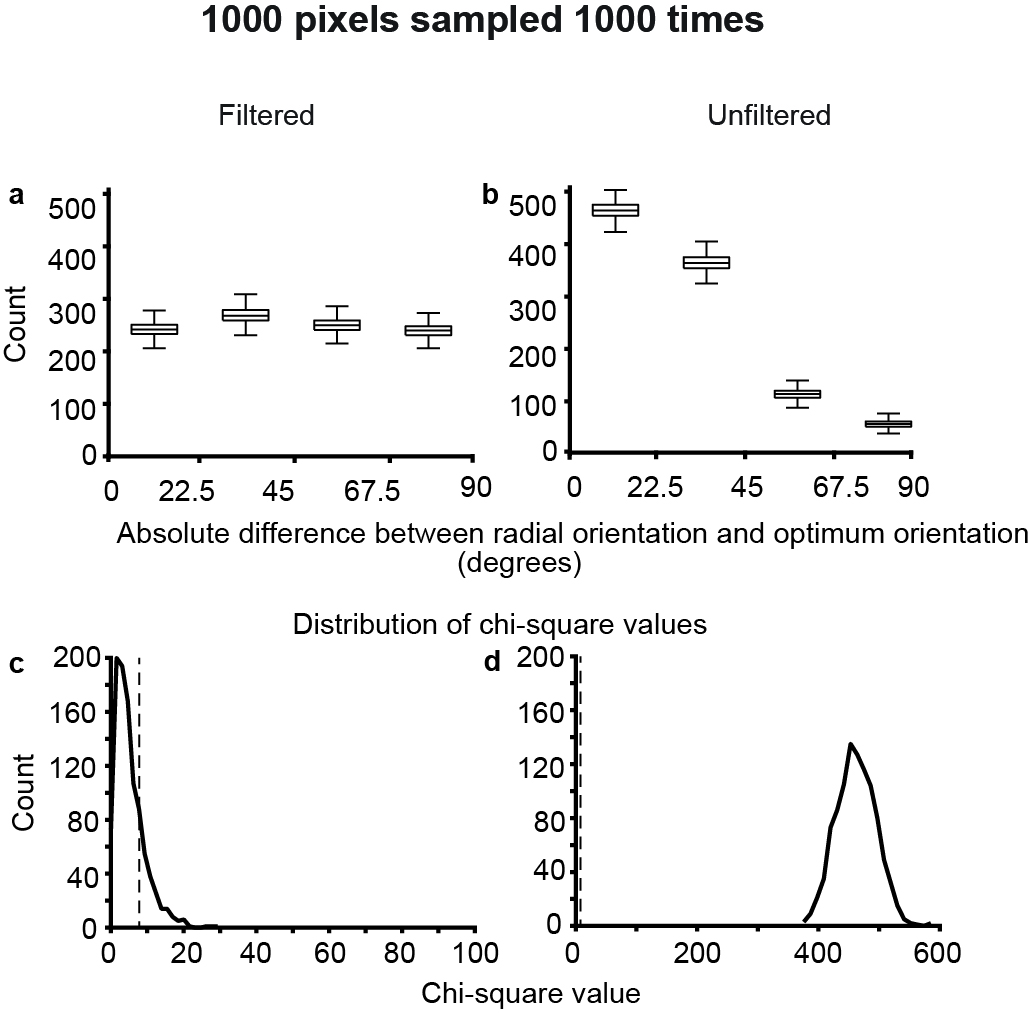
\includegraphics[width=\linewidth]{rb/FinalFigures/s4.jpg}
					\caption{Results of the random simulation experiment with 1000 pixels sampled 1000 times. See figure 6 for description of individual panels}
					\label{fig:s1000}
				\end{figure}
		\subsubsection{Orientation biases of the local field potentials}
		In two animals, we used single electrodes to record LFP as well as MUA from 6 recording sites. In one animal we used a multi-electrode array to record the LFP and MUA at a further 16 locations. The orientation tuning of the MUA and LFP of the array data are presented in figure 8. The multiunit activity changed consistently across subsequent electrodes so that most orientations were represented. The LFP activity on the other hand showed broader orientation tuning. Further, most sites were tuned to the radial orientation. The absolute differences between the optimum orientation of the LFP and the multiunit activity, and the radial angle of the imaged area are shown in figure \ref{fig:MUA} . This includes all 22 sites (from single electrodes and multi electrode arrays). A chi-squared test showed that the distribution of the differences of circular means of the LFP was significantly different from a uniform distribution (n=22;  $\chi^2$= 8.18; df=3; p=0.04) whereas the same was not true for the multi-unit activity (n=22;  $\chi^2$= 3.09; df=3; p=0.38).
				\begin{figure}[H]
					
					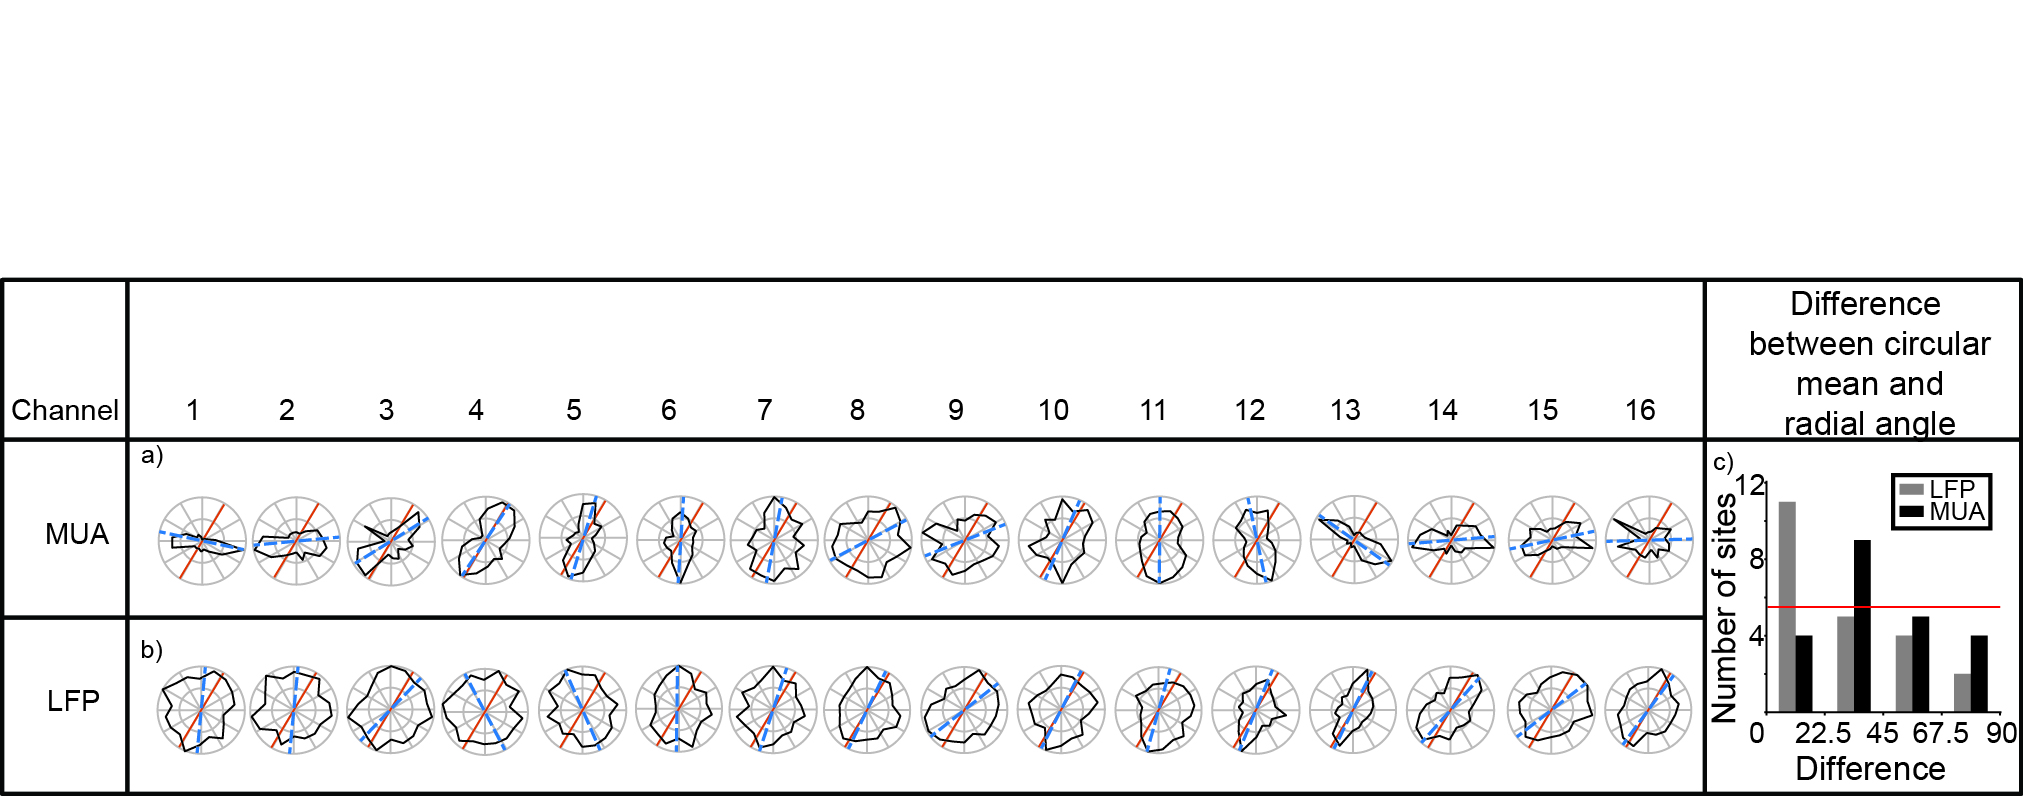
\includegraphics[width=\linewidth]{rb/FinalFigures/mua.jpg}
					\caption{Results of the random simulation experiment with 1000 pixels sampled 1000 times. See figure 6 for description of individual panels}
					\label{fig:MUA}
				\end{figure}
	
				\pagebreak
				
	\section{Discussion}
		
		Using optical imaging of intrinsic signals, we examined the OI signals at different spatial scales in the primary visual cortex of macaques. In a subset of animals, we also measured multi-unit responses and local field potentials in the primary visual cortex. We found that the large spatial scale signals in the OI and the LFP signals were tuned to the radial orientation while the smaller spatial scale signal and the multiunit responses did not show this preference for the radial angle. These results are consistent with the results from fMRI studies, where the BOLD signal is analogous to the OI haemodynamic signal, as well as the electrophysiological studies which show that in most animals studied, a radial bias exists in the visual system.
		
		During the experiment, we could have introduced systematic errors in various stages of data collection and analysis. The plotting of the foveal location is dependent on the visibility of the fovea when observed through the fundus camera. The visibility of the fovea itself is dependent on the optics which tend to deteriorate as the experiment progresses. During the experiment, we were able to more accurately characterise the optic nerve head. As a result, both the optic nerve and the first foveal position needed to be accurately plotted for us to accurately determine the radial angle. An error in plotting either of these parameters could lead to inaccurate estimation of the radial angle.
		
		Receptive field estimation is also subject to error. Within a track, there is a jitter of approximately half a degree in both receptive field position and size of the receptive field (Dow et al., 1981). Further, we also only used the receptive field position of the first unit encountered in each track. This was to make sure that the angle of the electrode to the surface did not affect the measurement of receptive field location. This compared with the fact that the ROI centres are extrapolated from the RF measurements could introduce another element of error in our radial angle estimates. The formula used for extrapolation, though standardised, may not be exactly accurate in every animal. Large variances in topography between individual animals (eg: See Dow et al., 1981) have been reported in macaques which could further compound the error in radial angle estimates.
		
		Further, the single pixel optimum orientations were all compared to the mean radial angle of the imaged area. The radial angles of the receptive fields in the imaged area can vary up to 30 degrees depending on the eccentricity of the receptive fields in the imaged area. This introduces a further element of error in the measurements which contribute to a larger spread of differences in the single pixel data. Taking into account all these sources of error in determining the difference between the radial angle and optimum orientation, the actual radial bias in the data may be stronger than has been reported.
		
		
		In our study, we have shown that the larger spatial scale activity is tuned to the radial orientation. However, the question of what these signals represent remains. The large spatial scale, global signal has been attributed to local blood flow and blood volume changes in the imaged area (Stetter et al., 2000; Pouratian and Toga, 2002). However, studies have shown that blood flow is also affected by neuronal activity through glial cells (Atwell et al., 2010), indicating that the blood volume changes accompany neuronal activity. One explanation lies in the fact that the BOLD responses (and therefore OI signals) are correlated with the LFP responses (Logothetis et al., 2001). This relationship is also demonstrated in our study, where the LFP and the ‘global’ OI signal were both predominantly tuned to the radial orientation. While the exact nature of the LFP signal is still not understood, general consensus is that this signal represents the synaptic, pre-synaptic and multi-unit observed in the recorded region of cortex and does not correspond well with the multi-unit activity (Berens et al., 2008; Logothetis et al., 2001). We propose that the larger spatial scale, global signal also corresponds with the pre-synaptic, synaptic and multi-unit activity. By removing the higher magnitude, larger spatial scale signals using a band-pass filter, optical imaging studies help isolate the responses that correspond to the scale of the multiunit activity. Therefore, the large spatial scale signal in the OI response corresponds to the synaptic and pre-synaptic activity, which reflect the tuning of the inputs to the imaged area. Our results indicate that the inputs to the primary visual cortex are tuned to the radial orientation.
	
		During imaging, the tandem lens arrangement allows us to focus on a very narrow plane under the surface of the cortex while imaging (Frostig et al.,1990). In this study, we focussed the tandem lens setup between 550-700 microns below the cortical surface. This depth corresponds to the region of the cortex just above the interface between Layer 3 and Layer 4. Unlike the cat Area 17, most neurons in the macaque layer 4 show broad orientation tuning, with sharp orientation emerging in Layers 2 and 3 for the first time (Bullier and Henry, 1980). Further, the areas of layers 2 and 3 that were imaged also receive direct inputs from konio-cellular layers of the LGN (Klein et al., 2016). This indicates that the cells in the imaged layer, like their layer 4 counterparts show broad orientation selectivity. Therefore, despite the depth where the camera was focussed and images were obtained from, we can conclude that the inputs to the cortex are tuned to the radial orientation.
	
		A previous study from our lab showed that inputs to neurons in the primary visual cortex were tuned to the same orientation as the orientation column to which they project (Vidyasagar et al., 2015). These results are not entirely contradictory to the results from our current study. Apart from any species differences that may be present, the earlier study showed a considerable jitter in the relationship between the orientation of the LGN fibres and cortical columns (r= 0.63). In our study, while the majority of the ROIs and pixels  in the unfiltered maps were tuned to the radial angle, there were also a proportion that were tuned betweem 22.5 and 90 degrees away from the radial angle. This departure from the radial angle is similar to that shown in the earlier study (Vidyasagar et al., 2015). 
		
		If the inputs to the primary visual cortex are tuned to the radial orientation, then this has some implications for orientation selectivity in the primary visual cortex. The theory of excitatory convergence for the generation of orientation selectivity was first proposed by Hubel and Wiesel (1962) and proposed that thalamic neurons with circular receptive fields arranged in a row converged on a striate cortical neuron to endow on it sharp orientation selectivity. This model assumption that thalamic neurons are untuned to orientation. Contrary to this belief, many studies have shown that subcortical neurons are indeed biased for orientation (Hammond, 1974; Levick and Thibos, 1980; Vidyasagar and Urbas, 1982; Leventhal, 1983; Van Hooser et al., 2013Vidyasagar and Henry, 1990; Smith et al., 1990; Passaglia et al., 2003; Shou and Leventhal, 1989; Sun et al., 2016). Our study adds to this extensive literature on sub-cortical biases by studying the organisation of the orientation selectivity of the inputs in the cortex, suggesting that most of these inputs are tuned to just one orientation. This provides support for a model of orientation selectivity where the inputs to the cortex arrive in a small number of broadly tuned orientation channels, from which the whole range of orientations observed in the primary visual cortex are generated (Vidyasagar and Eysel, 2015).
		
		Vidyasagar and Eysel (2015) proposed that all orientations in the cortex can be generated by broadly tuned orientation channels with orthogonal orientations. However, our study only shows a bias for the radial angle in the inputs to the cortex. orientations. This does not necessarily mean that only one orientation is present in the inputs. The large magnitude of the radial bias signal could mean that any smaller signals maybe masked. There are no ways to separate these signals on a spatially (as is usually done in the case of extracellular signals) without losing the information. Even if only one clear bias is present in the inputs, the cortex may still be able to generate all orientations. For example, phase selectivity is completely dominated by one polarity (75\% of neurons respond to light off; Albus and Wolf, 1984) in kittens but the cortical networks generates both on and off neurons from these limited inputs (Xin et al., 2008). In colour vision too, normal colour vision can be achieved even though there are only a relatively small proportion of S cones and large variation in the proportion of L and M cones (Kremers et al., 2000).
	
		Our study also highlights the importance of studying the optical imaging signal at different spatial scales as has been previously shown in cats, humans and macaques (Swisher et al., 2010; Tanigawa et al., 2017). In this study, we also highlight the use of optical imaging of intrinsic signals in studying the organisation of cortical inputs on a larger spatial scale. Future study can further characterise this large spatial scale, global signal which may be useful in determining organisation of inputs to the cortex.
		\pagebreak
	\section{Conclusion}
	
		In this chapter, we aimed to examine the large spatial scale activity in orientation maps to characterise radial bias in the optical imaging signal. We compared the optimum orientations of single pixels and ROIs to their radial angles and found that in the unfiltered maps, there was a prominent bias for the radial angle. The ROIs in the filtered maps showed a weaker bias for the radial orientation but no such bias was observed in the single pixel responses. We propose that these signals reflect the orientation tuning of the inputs to the cortex. If the majority of the inputs to the cortex are indeed tuned to the radial angle, then this provides evidence for a model of orientation selectivity where orientation input arriving in a small number of broadly tuned channel are further sharpened in the primary visual cortex to generate the whole range of orientation preferences observed in the cortex. 
		